\documentclass[a4paper,11pt]{article}
\usepackage{graphicx}
\usepackage{booktabs}
\usepackage{setspace}
\usepackage{parskip}
\usepackage[english]{babel}
\usepackage{refstyle}
\usepackage{hyperref}
\usepackage{caption}
\usepackage{subcaption}
\onehalfspacing
\begin{document}

\author{Mario Tambos}
\title{\vspace{-2cm}Report for Sheet 01\\
\small{Lab Course Machine Learning and Data Analysis}}
\maketitle

\section*{Implementation comments}
The code was structured mostly in functions following an imperative paradigm,
except for the \verb|PCA| class, which was required by the assignment's statement.

One function was declared for each assignment in Part 2.

Given the low time performance of the LLE's implementation for the assignment,
it was decided to use \verb|scikit-learn|'s \verb|LocallyLinearEmbedding|
class for Assignment 8, in order to optimize the $k$ hyperparameter
more quickly.

Beyond \verb|matplotlib|, \verb|numpy| and \verb|scipy|, \verb|networkx| was
used to build and display the node neighborhood graphs, \verb|tqdm| to show
progress bar on loops, and \verb|pandas| together with \verb|seaborn| to show
the boxplots in Assignment 6.

All tasks were completed. However, the denoising test failed in Assignment 1,
and no good value for $k$ could be found in Assignment 8 for the high noise case.

In the denoising case, the cause of the failure is unclear. The result's provided
by the exercise's \verb|PCA| implementation were successfully checked against
results from the \verb|scikit-learn|'s \verb|PCA| class.

In the high-noise case in Assignment 8, the problems seems to be that there is no
right $k$ value. For low values of $k$, all points are embedded in a very small
interval. For larger values of $k$, the points use neighbors from the inner loops
of the spiral to calculate the embedding, resulting in something similar to the
bottom plot in \figref{assignment5-2-b-abc}.
\section*{Assignment 5}
\subsection*{2)}
\subsubsection*{b)}

\Figref{assignment5-2-b-abc} shows the result of performing PCA on the \verb|usps| dataset.

\begin{figure}
  \centering
  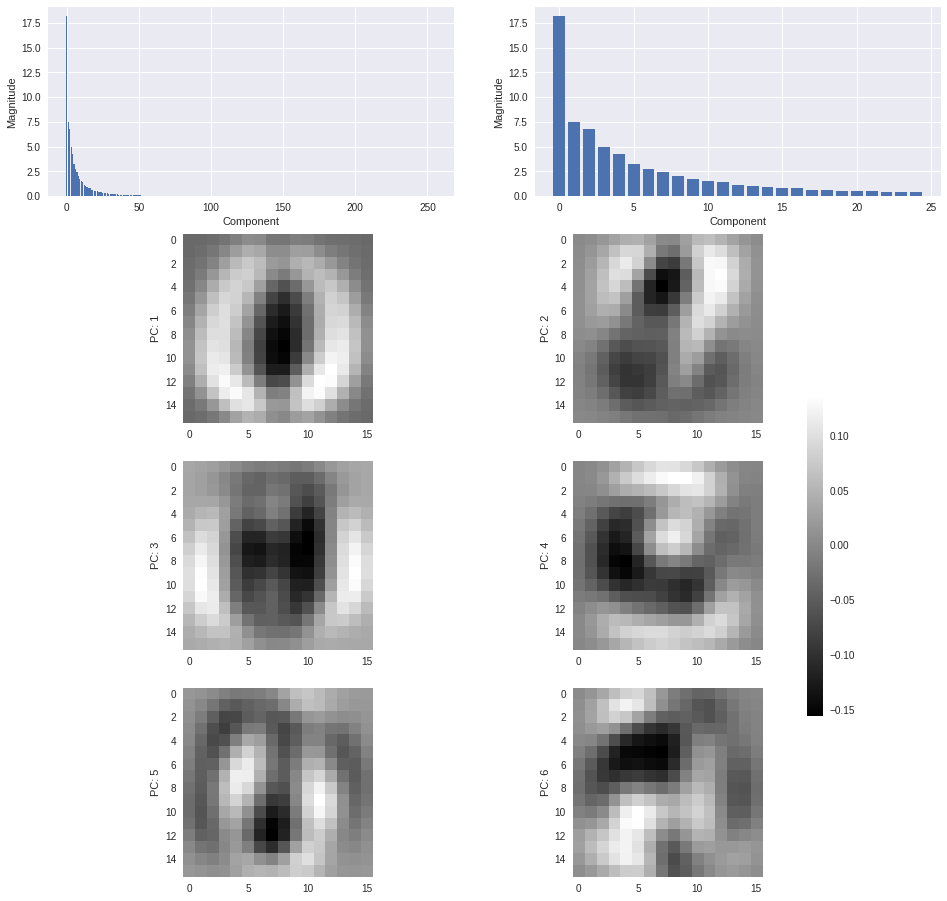
\includegraphics[width=\textwidth]{images/assignment5-2-b-abc.png}
  \caption{PCA for the \texttt{usps}  dataset. The top left plot shows all principal values extracted, while the top right plot shows only the first (largest) 25 values. The bottom 6 images show the first 6 principal directions.}
  \label{fig:assignment5-2-b-abc}
\end{figure}

\subsection*{3)}

The most notable differences when contrasting \figref{assignment5-2-b-abc} against \figref{assignment5-3-lgn1,assignment5-3-hgn1,assignment5-3-out1} are the resulting principal components. The only other noticeable difference is the higher magnitude
of the smallest eigenvalues in the high noise scenario.

As expected, the reconstructions in \figref{assignment5-3-lgn2} are better than in \figref{assignment5-3-hgn2}. In the outliers scenario (\figref{assignment5-3-out2}),
the reconstructions were surprisingly good for the outliers, but the reconstructions
of the images without noise were comparable to \figref{assignment5-3-hgn2}.

\subsubsection*{Low Gaussian noise}

The experiment results for the scenario where Gaussian noise drawn from $\mathcal{N}(0, \sigma^2=0.3)$ was added is shown in \figref{assignment5-3-lgn}.

\begin{figure}
	\centering
	\begin{subfigure}[t]{0.45\textwidth}
		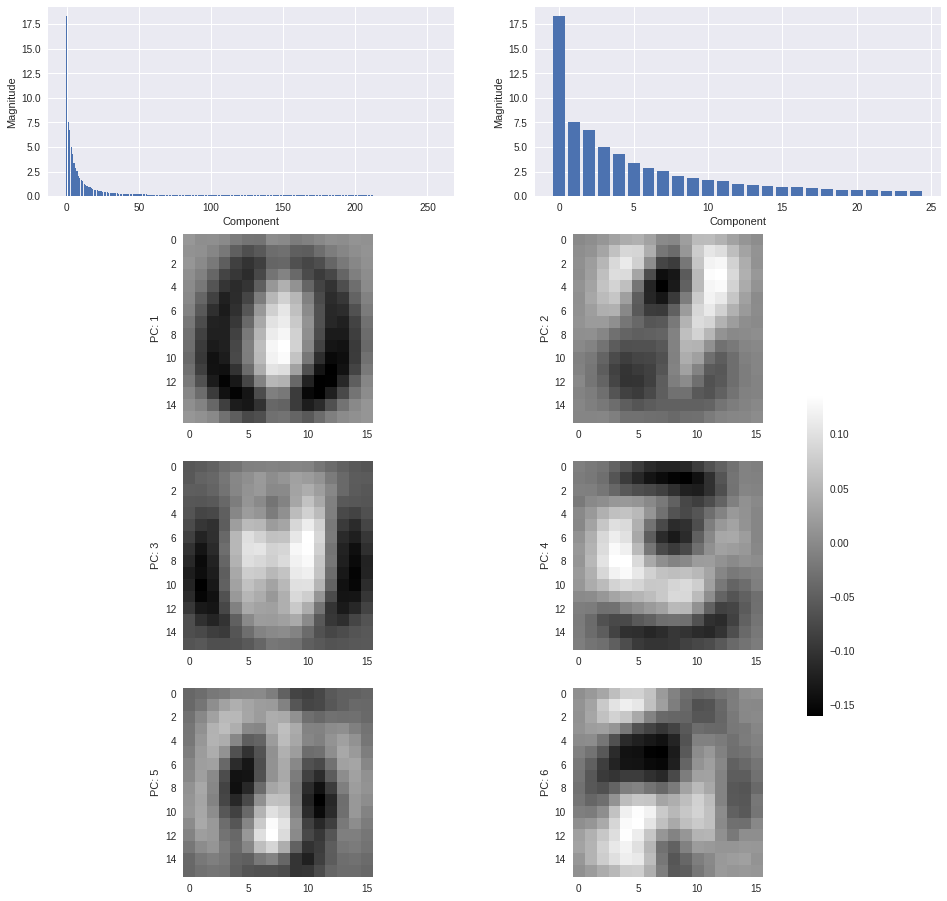
\includegraphics[width=\textwidth]{images/assignment5-3-lgn1.png}
		\caption{The top left plot shows all principal components, while the top right plot shows only the first 25 components. The bottom 6 images show the first 6 principal directions.}
		\label{fig:assignment5-3-lgn1}
	\end{subfigure}
	\hfill
	\begin{subfigure}[t]{0.45\textwidth}
		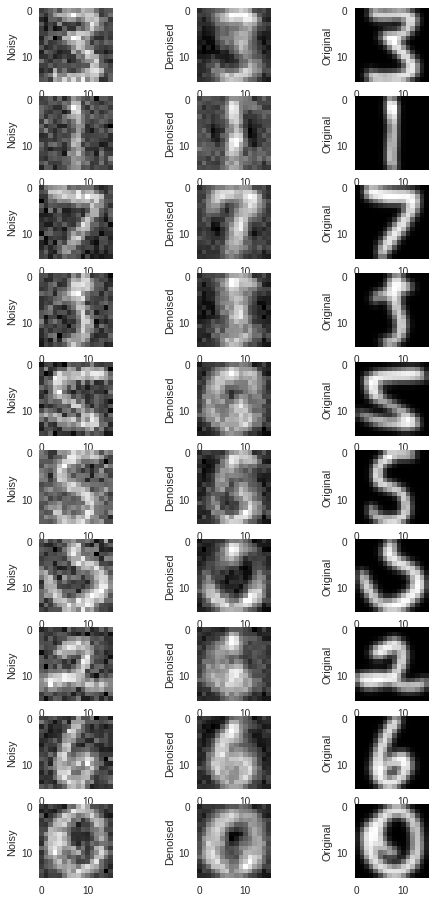
\includegraphics[width=\textwidth]{images/assignment5-3-lgn2.png}
		\caption{Random sample of 10 items. The first column shows the noisy versions, the middle column the denoised versions (using PCA) and the last column shows the original images.}
		\label{fig:assignment5-3-lgn2}
	\end{subfigure}
	\caption{PCA denoising. Low Gaussian noise ($\sigma=0.3$) scenario.}
	\label{fig:assignment5-3-lgn}
\end{figure}

\subsubsection*{High Gaussian noise}

The experiment results for the scenario where Gaussian noise drawn from $\mathcal{N}(0, \sigma^2=0.7)$ was added is shown in \figref{assignment5-3-hgn}.

\begin{figure}
	\centering
	\begin{subfigure}[t]{0.45\textwidth}
		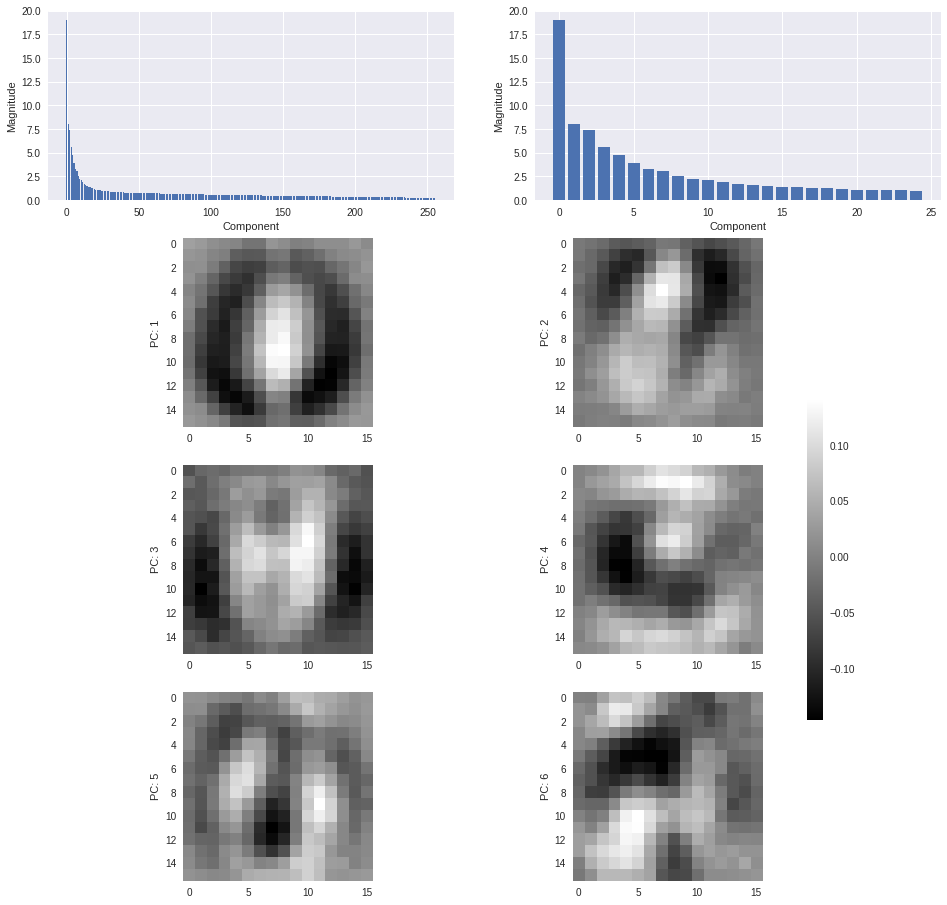
\includegraphics[width=\textwidth]{images/assignment5-3-hgn1.png}
		\caption{The top left plot shows all principal components, while the top right plot shows only the first 25 components. The bottom 6 images show the first 6 principal directions.}
		\label{fig:assignment5-3-hgn1}
	\end{subfigure}
	\hfill
	\begin{subfigure}[t]{0.45\textwidth}
		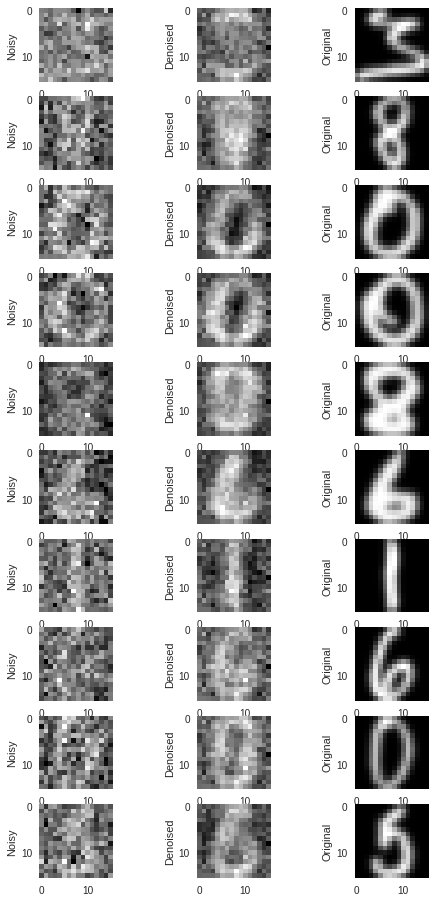
\includegraphics[width=\textwidth]{images/assignment5-3-hgn2.png}
		\caption{Random sample of 10 items. The first column shows the noisy versions, the middle column the denoised versions (using PCA) and the last column shows the original images.}
		\label{fig:assignment5-3-hgn2}
	\end{subfigure}
	\caption{PCA denoising. High Gaussian noise ($\sigma=0.7$) scenario.}
	\label{fig:assignment5-3-hgn}
\end{figure}

\subsubsection*{Outliers}

The experiment results for the scenario where Gaussian noise drawn from $\mathcal{N}(0, \sigma^2=5)$ was added to the first five images is shown in \figref{assignment5-3-out}.

\begin{figure}
	\centering
	\begin{subfigure}[t]{0.45\textwidth}
		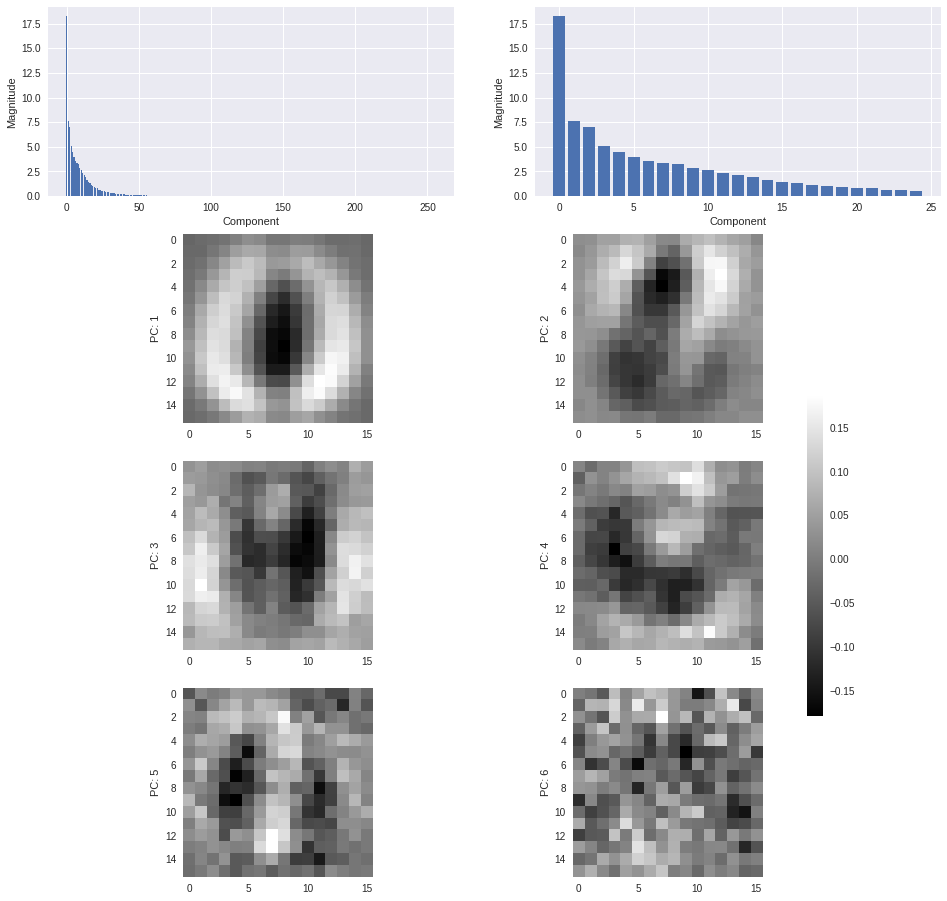
\includegraphics[width=\textwidth]{images/assignment5-3-out1.png}
		\caption{The top left plot shows all principal components, while the top right plot shows only the first 25 components. The bottom 6 images show the first 6 principal directions.}
		\label{fig:assignment5-3-out1}
	\end{subfigure}
	\hfill
	\begin{subfigure}[t]{0.45\textwidth}
		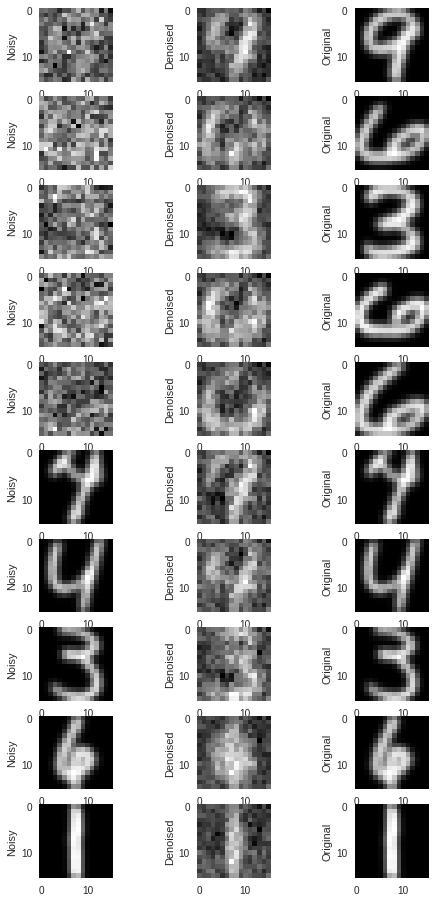
\includegraphics[width=\textwidth]{images/assignment5-3-out2.png}
		\caption{Random sample of 10 items. The first column shows the noisy versions, the middle column the denoised versions (using PCA) and the last column shows the original images.}
		\label{fig:assignment5-3-out2}
	\end{subfigure}
	\caption{PCA denoising. Outliers (~$\mathcal{N}(0, \sigma=5)$ added to the first 5 images) scenario.}
	\label{fig:assignment5-3-out}
\end{figure}

\section*{Assignment 6}


\Figref{assignment6} shows the experiment's results in three boxplots. The
$\gamma$-index method with $k=3$ performed consistently better than with $k=5$, but
both were outperformed by the distance-to-the-mean method in all cases.
Moreover, the confidence intervals of the three methods were tighter the higher the
outlier rate.

\begin{figure}
	\centering
	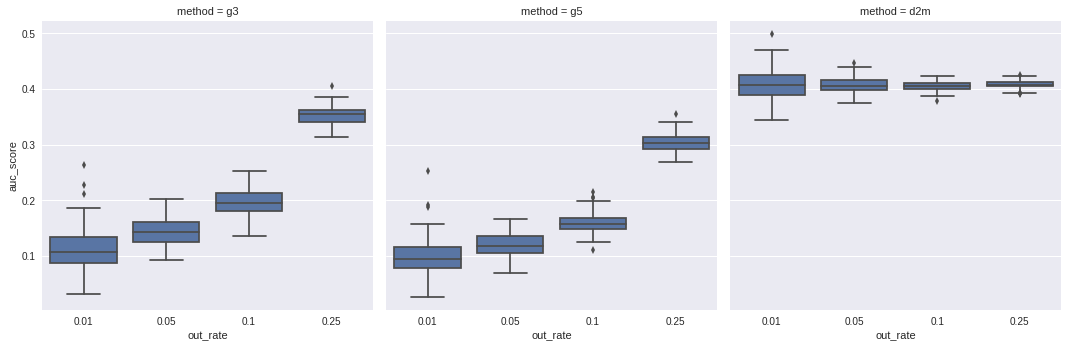
\includegraphics[width=\textwidth]{images/assignment6.png}
	\caption{Outlier detection AUC scores on the \texttt{banana} dataset.
			 The leftmost plot shows the AUC scores using the $\gamma$-index
			 method with $k=3$.
		     The middle plot shows the AUC scores using the $\gamma$-index
		     method with $k=5$.
	         The rightmost plot shows the AUC scores using the
	         distance-to-the-mean method.
	         The x-axis indicates the outlier rate used ($0.01$, $0.05$,
	         $0.1$ and $0.25$).}
	\label{fig:assignment6}
\end{figure}

\section*{Assignment 7}

\Figref{assignment7} shows the 1-D and 2-D LLE projections for the \verb|fishbowl|, \verb|swissroll| and \verb|flatroll| datasets.

\begin{figure}
	\centering
	\begin{subfigure}[b]{\textwidth}
		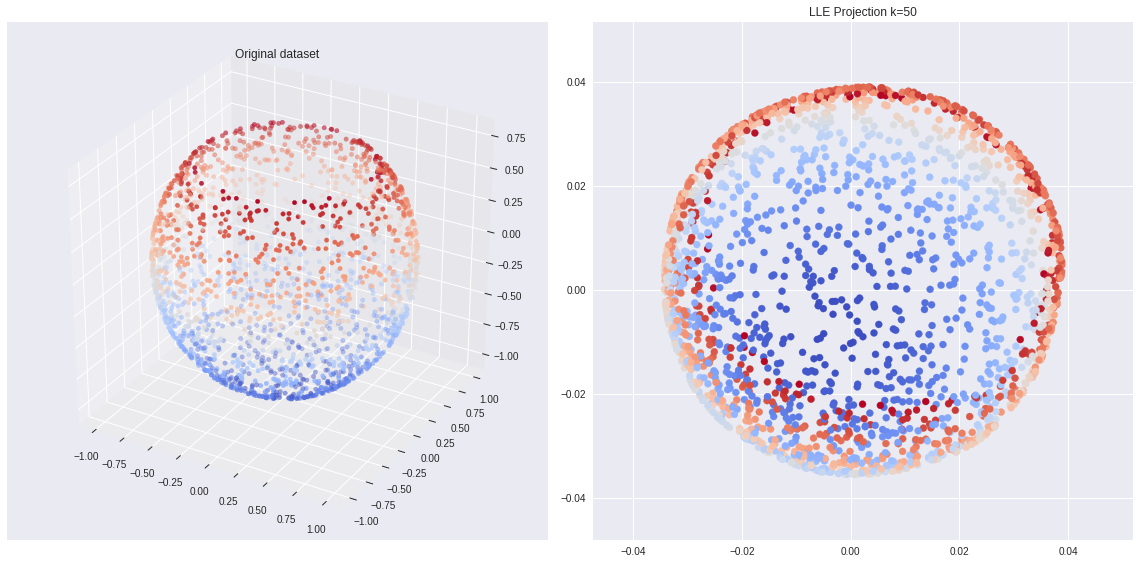
\includegraphics[width=0.9\textwidth]{images/assignment7-1.png}
		\caption{2-D LLE projection for the \texttt{fishbowl} dataset.
				 Right: original; left: projection.
				 Method used: k-nearest-neighbors; $k=50$}
		\label{fig:assignment7-1}
	\end{subfigure}
	\\
	\begin{subfigure}[b]{\textwidth}
		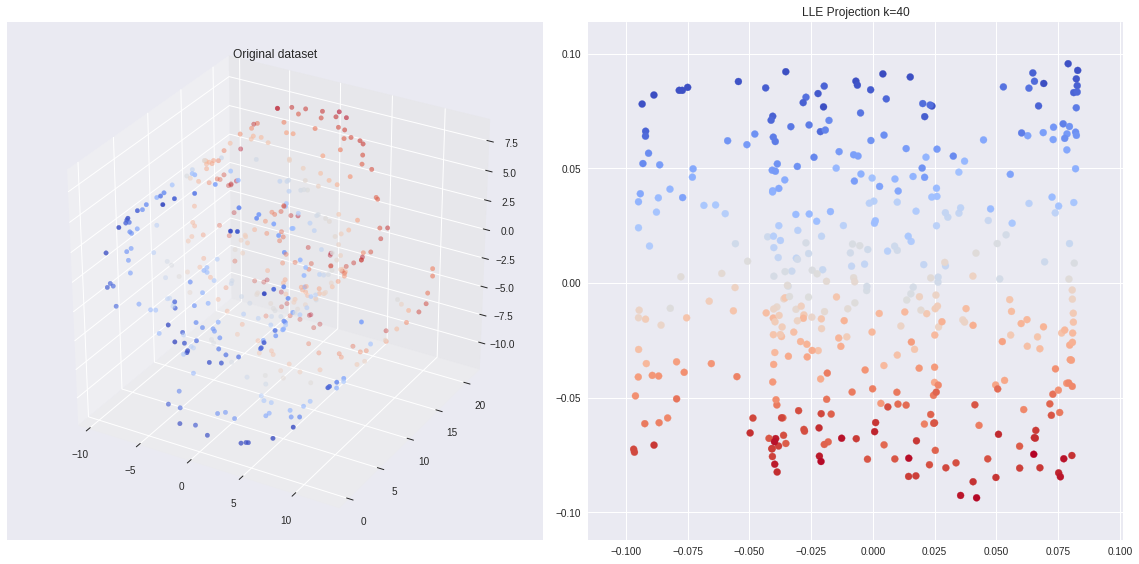
\includegraphics[width=0.9\textwidth]{images/assignment7-2.png}
		\caption{2-D LLE projection for the \texttt{swissroll} dataset.
				 Right: original; left: projection.
				 Method used: k-nearest-neighbors; $k=40$}
		\label{fig:assignment7-2}
	\end{subfigure}
	\\
	\begin{subfigure}[b]{\textwidth}
		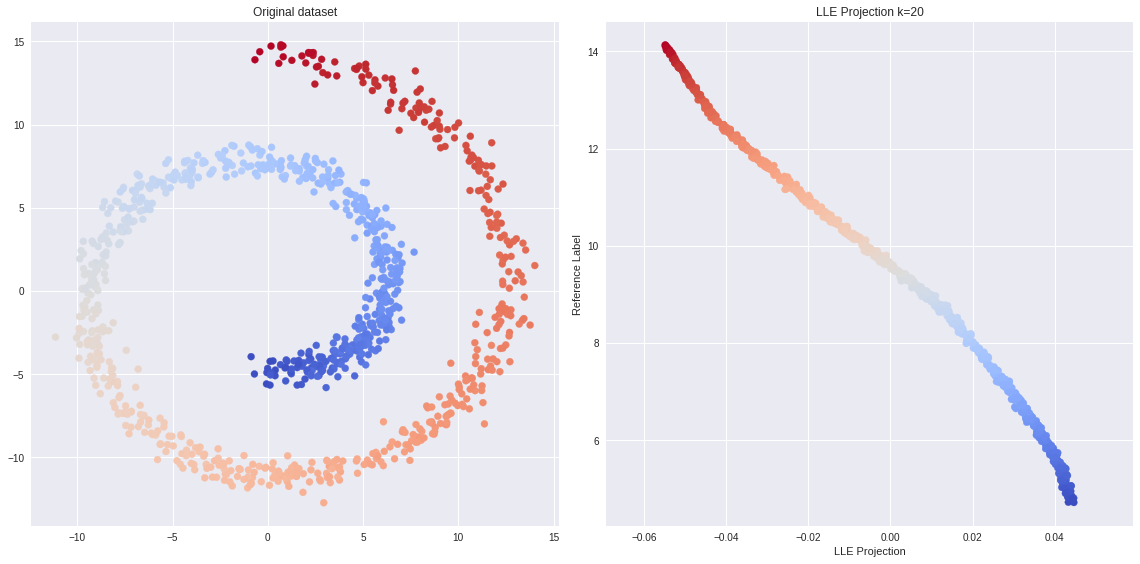
\includegraphics[width=0.9\textwidth]{images/assignment7-3.png}
		\caption{1-D LLE projection for the \texttt{flatroll} dataset.
				 Right: original; left: projection.
				 Method used: k-nearest-neighbors; $k=20$}
		\label{fig:assignment7-3}
	\end{subfigure}
	\caption{LLE projections.}
	\label{fig:assignment7}
\end{figure}
\section*{Assignment 8}

\Figref{assignment7} shows the 1-D LLE projections for the \verb|flatroll| dataset, in which Gaussian noise drawn from $\mathcal{N}(0, \sigma=0.2)$ and $\mathcal{N}(0, \sigma=1.8)$ was added.

\begin{figure}
	\centering
	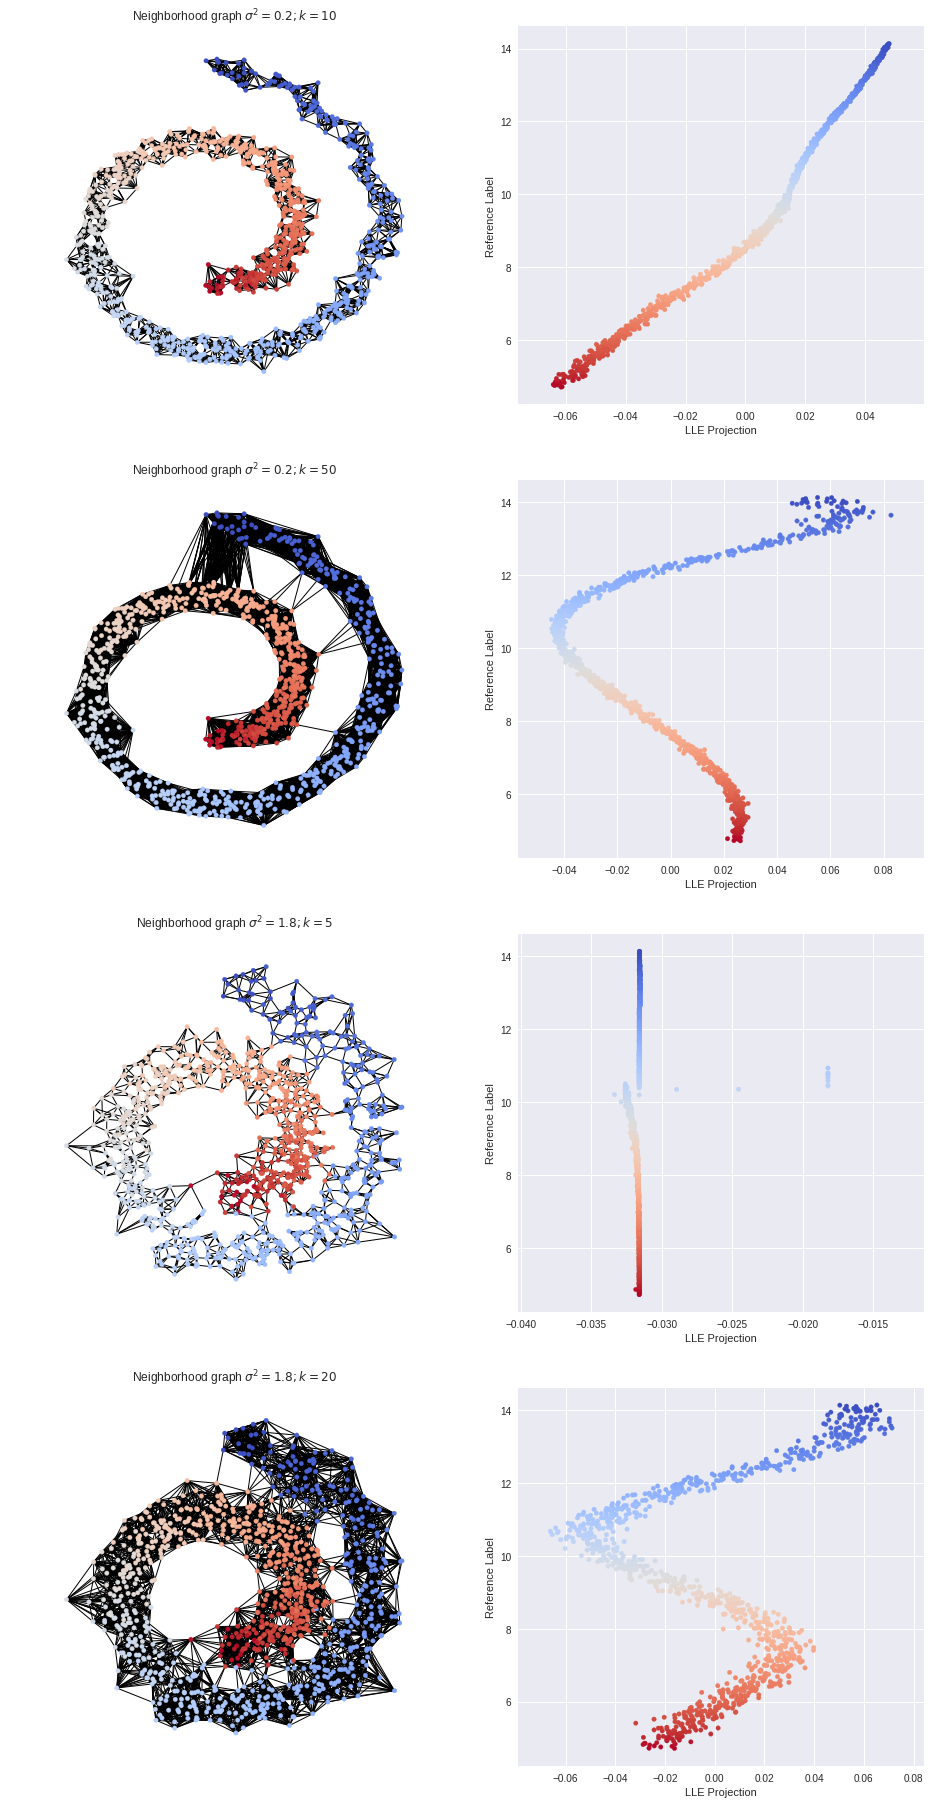
\includegraphics[height=0.85\textheight]{images/assignment8.png}
	\caption{1-D LLE projections for the \texttt{flatroll} dataset + Gaussian noise.
			 The top two plots show the dataset + $\mathcal{N}(0, \sigma^2=0.2)$;
			 with the topmost one using parameter $k=10$ and the following one
			 using $k=50$.
			 The bottom two plots show the dataset + $\mathcal{N}(0, \sigma^2=1.8)$;
			 with the upper one using parameter $k=5$ and the following one using
			 $k=20$.
		 }
	\label{fig:assignment8}
\end{figure}

\end{document}

